

\section{CPU or network saturation}

Target: see what is the bottleneck in JPaxos - network or CPU?

Measured: cpu and network usage on leader, follower and client machine.

\subsection{1024B requests}

\subsubsection{CPU}
\strut

Iddle CPU on nodes [percentage]:\\
{\ttfamily
\begin{tabular}{|r|c|c|c|}\hline
/ & Client & Follower & Leader \\ \hline
0 & 89,60  & 69,57    & 58,67  \\ \hline
1 & 89,16  & 80,12    & 57,95  \\ \hline
2 & 86,34  & 89,32    & 67,76  \\ \hline
3 & 64,52  & 60,87    & 37,45  \\ \hline
\end{tabular}         
}

\medskip

Leader and follower average CPU detailed usage:\\
{\ttfamily
\begin{tabular}{|c|c|c|c|c|c|c|}\hline
          &  user  &   sys  & iowait & irq   & soft  & idle  \\ \hline
leader:   & 23,92  &  10,13 & 0,07   & 1,77  & 8,66  & 55,46 \\ \hline
follower: & 14,51  &  04,71 & 0,12   & 1,06  & 4,62  & 74,97 \\ \hline
\end{tabular}
}

\medskip

Leader per-core CPU detailed usage:\\
{\ttfamily
\begin{tabular}{|c|c|c|c|c|c|c|c|}\hline
CPU & user   & sys   & iowait& irq  &  soft  &  idle  \\ \hline
0   & 31,25  & 8,27  & 0,00  & 0,00 &  1,81  &  58,67 \\ \hline
1   & 30,08  & 9,55  & 0,00  & 0,00 &  2,42  &  57,95 \\ \hline
2   & 18,26  & 11,22 & 0,00  & 0,00 &  2,76  &  67,76 \\ \hline
3   & 16,09  & 11,47 & 0,28  & 7,06 &  27,66 &  37,45 \\ \hline
\end{tabular}
}

\medskip

{\small Legend:\\
\begin{tabular}{rl}
user & executing at the user level (application)\\
 sys & executing at the system level (kernel) without any interrupts\\
 irq & hardware interrupts\\
soft & software interrupts\\
\end{tabular}
}

\paragraph{Conclusions}
CPU is not saturated.
Thread CPU usage is unbalanced.
Thread performing network tasks uses processor at most.
If the throughput would increase by 60\%, the CPU would be a possible bottleneck.

New test needed: how small must the request size be to saturate CPU.

\subsubsection{Network}

Used bandwidth on nodes [10\textasciicircum 6bits/s aka Mbit/s]:

\begin{tabular}{|r|c|c|c|}\hline
 /  & Client & Follower & Leader \\ \hline
in  & 130    & 484      & 394    \\ \hline
out & 128    & 215      & 908    \\ \hline
\end{tabular}

Measured TCP throughput on the network is 941.07 [10\textasciicircum 6bits/s] (3× \texttt{netperf -H hpc3 -cC -fm -j -tTCP\_STREAM -\strut- -m 1024}).
Bandwidth used during the test TCP throughput test is 987 [10\textasciicircum 6bits/s].

\paragraph{Conclusions}
Network usage reaches 92\% of its capabilities. This means that the network is close to saturation, yet not fully saturated.
Network is a bottleneck in this test.

% TODO: request size / bandwidth

\subsection{Multiple request sizes}

Following test shows how JPaxos behaves with 16B, 128B, 1024B and 8196B requests.\\
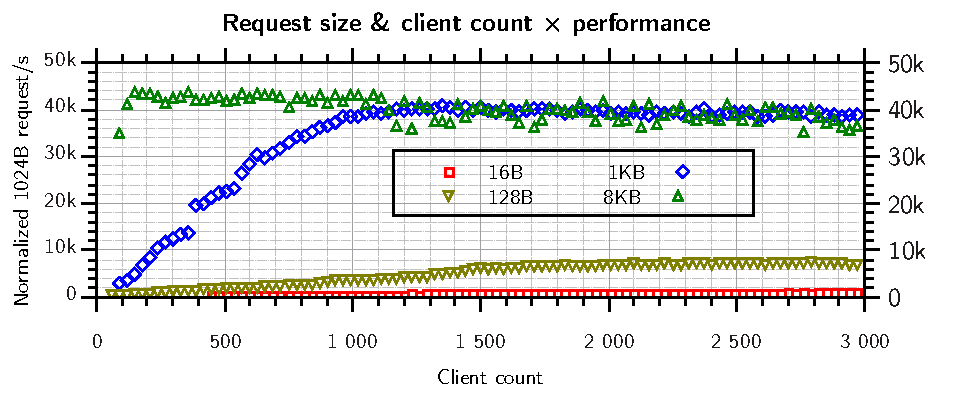
\includegraphics{varia/reqSize-cliCount}

The values on the plot are normalized, i.e., 8KB request count per second has been multiplied by 8, and the 128B request count per second has been divided by 8. This makes the results comparable.

With 8KB requests the network gets saturated very soon (with 150 clients).
With 1KB requests the network gets saturated starting from 1200 clients.
Smaller requests cannot saturate the network, and after reaching peek throughput at about 2500 clients, the performance drops.

\bigskip

To see when the border request byte size where JPaxos stops saturating CPU and starts saturating network, the following test has been done:
 \begin{itemize}
 \item 3×700 clients
 \item request size varying from 16B to 2048B
\end{itemize}

The results, unnormalized, are as follows:\\
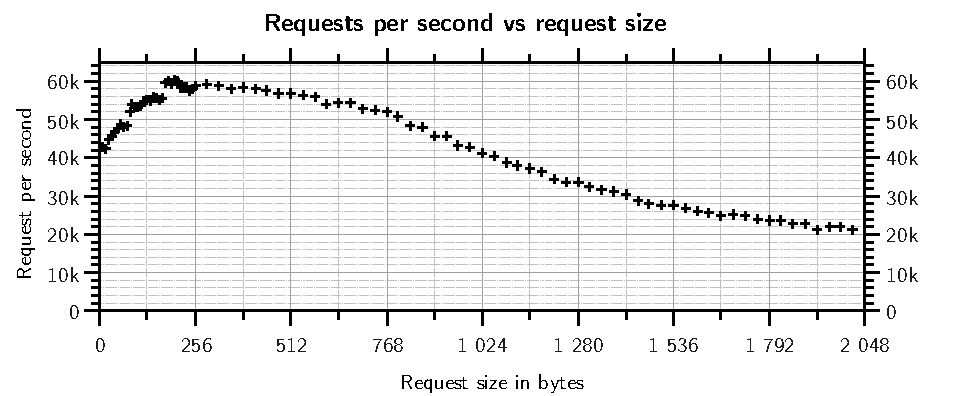
\includegraphics{varia/reqSize_reqs.pdf}

So to get highest request per second value (in order to show 'we have the highest r/s'), one must take 200B requests.
This however says nothing about real performance.

\medskip

Following plot shows state-machine level goodput (i.e. how much data the state machine got in a time unit):\\
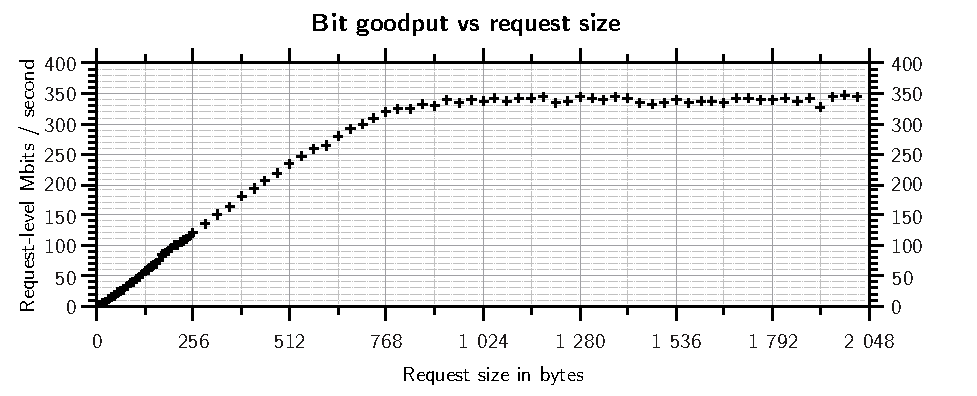
\includegraphics{varia/reqSize_mbps.pdf}

The plot shows that when the request size exceeds about 900B, the network gets saturated. 
Up to 768 bytes the bit throughput grows nearly linearly with increasing request size -- larger request takes the same CPU time, but transports more data. Starting from about 900B the number of requests per second decreases, but the amount of data remains on a stable level, indicating ghat the network bandwidth limits throughput.

The test included 2100 clients total, which is enough to produce an amount of request needed to saturate the network from clients to the replicas starting with request size of 180B (in theory), so increasing the number of client won't change the 
900B limit.


\subsection{200B requests}

After analysing various request sizes, 200B requests were taken under account:

\subsubsection{Network}

Used bandwidth on nodes [10\textasciicircum 6bits/s aka Mbit/s]:\\
\begin{tabular}{|r|c|c|c|}\hline
 /  & Client & Follower & Leader \\ \hline
in  & 57     & 172      & 136    \\ \hline
out & 52     & 99       & 297    \\ \hline
\end{tabular}

There is a lot of bandwidth free. Less than 1/3rd of bandwidth is used on any machine in any single direction. Network is not the bottleneck.

\subsubsection{CPU}

Iddle CPU on nodes [percentage]:\\
{\ttfamily
\begin{tabular}{|r|c|c|c|}\hline
/ & Client & Follower & Leader \\ \hline
0 & 81,66  & 50,03    & 43,72  \\ \hline
1 & 82,75  & 54,90    & 36,86  \\ \hline
2 & 79,96  & 81,70    & 62,68  \\ \hline
3 & 55,98  & 68,00    & 46,98  \\ \hline
\end{tabular}         
}

All machines have higher CPU usage, but there is still a lot of free time on any node. (?)

\medskip

Leader and follower average CPU detailed usage:\\
{\ttfamily
\begin{tabular}{|c|c|c|c|c|c|c|}\hline
          &  user  &   sys  & iowait & irq   & soft  & idle  \\ \hline
leader:   & 33,09  & 12,12  & 0,09   & 0,83  & 6,16  & 47,4  \\ \hline
follower: & 24,86  &  7,63  & 0,17   & 0,51  & 3,17  & 63,66 \\ \hline            
\end{tabular}
}

\medskip

Leader per-core CPU detailed usage:\\
{\ttfamily
\begin{tabular}{|c|c|c|c|c|c|c|c|}\hline
CPU & user   & sys   & iowait& irq  &  soft  & idle  \\ \hline
0   & 39,13  & 15,63 & 0,00  & 0,00 &  1,50  & 43,74 \\ \hline
1   & 51,78  & 10,23 & 0,00  & 0,00 &  1,07  & 36,91 \\ \hline
2   & 24,30  & 11,43 & 0,00  & 0,04 &  1,43  & 62,80 \\ \hline
3   & 17,14  & 11,18 & 0,35  & 3,36 & 20,95  & 47,03 \\ \hline
\end{tabular}
}

Leader has a lot to do, but there is free processor time left.

If not CPU and network, it seems that synchronisation issues slow down the JPaxos now. (I hope to have time to discuss it with Tadek and Maciej).